\chapter{Introduction}
Type random text here
\section{Motivation}
\textbf{Title:} Remote servicing of IPTV using DirectFB and VNC.

\subsection{Objectives}
Assume you have an IPTV in your home and it has some technical problem. It will be better if the TV technician can solve the problem remotely over Internet. 

\subsection{Methodology}
The project involves 2 primary objectives
\begin{enumerate}
\item Exploring VNC system module of DirectFB and building it onto the target IPTV
\item Extending remote accessibility of IPTV from outside LAN
\end{enumerate}

\subsection{Applications}
DirectFB features and VNC features have been implemented in IPTV independently.

\subsection{Advantages and Disadvantages}
The primary goal is establishing communication between IPTV and a remote PC for remote serviceability of IPTV.

\subsection{Organisation of the Report}

\subsubsection{IPTV}
	Internet Protocol television (IPTV) is a system through which Internet television services are delivered using the architecture and networking.\cite{IPTV}\\

\subsubsection{NXP\_TV550}
	NXP\_TV550 is a single chip LCD TV platform that allows viewers to enjoy HD digital television and internet content with excellent picture quality on mid-range televisions. This module has been provided by PHILIPS and the VNC server is to be ported on this module.\\


\subsection{Software tools available}
\subsubsection{VNC}
	VNC is a remote control software which lets you see and interact with desktop applications across any network. The software has a widespread user base from individuals to the multi-national companies.You can use VNC to view a Windows 7 desktop at the office on a Linux or Mac computer at home as shown in \fref{fig:vnc} \cite{VNC}\\

\begin{figure}[h]
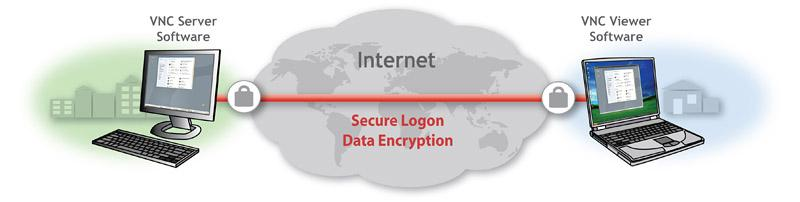
\includegraphics[scale=.5]{images/vnc.jpg}
\caption{VNC server-client model}\label{fig:vnc}
\end{figure}


\subsection{Project Organization}
	The project is split-up into 6 stages as shown in table :\\
	
\begin{tabular}{|c|c|c|}\hline
Sl No&Work& Duration(in Weeks)\\ \hline \normalsize
1&Information Collection on DFB \& VNC&1 \\ \hline
2&Information collection on development tools&2\\ \hline
3&Integrating DirectFB \& VNC&8\\ \hline
4&Cross Compiling \& Porting&2\\ \hline
5&Building JPEG libraries&2\\ \hline
6&Testing&2\\ \hline
\end{tabular}

\subsection{Project Execution}
We plan to work in these lines step-by-step
\begin{itemize}
\item Familiarize with dfb. Write simple applications. Try `windowed mode’ and `multi application mode’ on target running on X11 system module.
\item Ensure proper configuration and successful operation in these modes.
\item Run these applications on IPTV by booting from the root system on the
\item USB drive device. Control applications using putty.
\item Compile and explore fusion modules.
\item Explore vnc system module and how it provides interface options to libvnc

\end{itemize}
